\documentclass[11pt,a4paper,oneside]{report}

% thanks to http://tex.stackexchange.com/a/47579/71109
\usepackage{pdfpages}
\usepackage{ifxetex}
\usepackage{ifluatex}
\newif\ifxetexorluatex % a new conditional starts as false
\ifnum 0\ifxetex 1\fi\ifluatex 1\fi>0
   \xetexorluatextrue
\fi

\ifxetexorluatex
  \usepackage{fontspec}
\else
  \usepackage[T1]{fontenc}
  \usepackage[utf8]{inputenc}
  \usepackage[lighttt]{lmodern}
  \ttfamily\DeclareFontShape{T1}{lmtt}{m}{it}{<->sub*lmtt/m/sl}{}
\fi

\usepackage[english,magyar]{babel} % Alapértelmezés szerint utoljára definiált nyelv lesz aktív, de később külön beállítjuk az aktív nyelvet.

\usepackage{emptypage} % omit page number on empty pages

%\usepackage{cmap}
\usepackage{amsfonts,amsmath,amssymb} % Mathematical symbols.
%\usepackage[ruled,boxed,resetcount,linesnumbered]{algorithm2e} % For pseudocodes. % beware: this is not compatible with LuaLaTeX, see http://tex.stackexchange.com/questions/34814/lualatex-and-algorithm2e
\usepackage{booktabs} % For publication quality tables for LaTeX
\usepackage{graphicx}

%\usepackage{fancyhdr}
%\usepackage{lastpage}

\usepackage{anysize}
%\usepackage{sectsty}
\usepackage{setspace} % For setting line spacing

\usepackage[unicode]{hyperref} % For hyperlinks in the generated document.
\usepackage{xcolor}
\usepackage{listings} % For source code snippets.

\usepackage[amsmath,thmmarks]{ntheorem} % Theorem-like environments.

\usepackage[hang]{caption}

\singlespacing

\newcommand{\selecthungarian}{
	\selectlanguage{magyar}
	\setlength{\parindent}{2em}
	\setlength{\parskip}{0.5em}
	\frenchspacing
}

\newcommand{\selectenglish}{
	\selectlanguage{english}
	\setlength{\parindent}{0em}
	\setlength{\parskip}{0.5em}
	\nonfrenchspacing
	\renewcommand{\figureautorefname}{Figure}
	\renewcommand{\tableautorefname}{Table}
	\renewcommand{\partautorefname}{Part}
	\renewcommand{\chapterautorefname}{Chapter}
	\renewcommand{\sectionautorefname}{Section}
	\renewcommand{\subsectionautorefname}{Section}
	\renewcommand{\subsubsectionautorefname}{Section}
}

\usepackage[numbers]{natbib}
\usepackage{xspace}


\newcommand{\vikszerzoVezeteknev}{Fintha}
\newcommand{\vikszerzoKeresztnev}{Dénes Flórián}

\newcommand{\vikkonzulensAMegszolitas}{Dr.~}
\newcommand{\vikkonzulensAVezeteknev}{Bergmann}
\newcommand{\vikkonzulensAKeresztnev}{Gábor}

\newcommand{\vikkonzulensBMegszolitas}{}
\newcommand{\vikkonzulensBVezeteknev}{}
\newcommand{\vikkonzulensBKeresztnev}{}

\newcommand{\vikkonzulensCMegszolitas}{}
\newcommand{\vikkonzulensCVezeteknev}{}
\newcommand{\vikkonzulensCKeresztnev}{}

\newcommand{\vikcim}{Performance analysis of a language tooling}
\newcommand{\viktanszek}{\bmemit}
\newcommand{\vikdoktipus}{\bsc}
\newcommand{\vikmunkatipusat}{szakdolgozatot}

\input{include/tdk-variables}
\newcommand{\szerzoMeta}{\vikszerzoVezeteknev{} \vikszerzoKeresztnev}
\input{include/thesis-en}
%--------------------------------------------------------------------------------------
% Page layout setup
%--------------------------------------------------------------------------------------
% we need to redefine the pagestyle plain
% another possibility is to use the body of this command without \fancypagestyle
% and use \pagestyle{fancy} but in that case the special pages
% (like the ToC, the References, and the Chapter pages)remain in plane style

\pagestyle{plain}
\marginsize{35mm}{25mm}{15mm}{15mm}

\setcounter{tocdepth}{3}
%\sectionfont{\large\upshape\bfseries}
\setcounter{secnumdepth}{3}

\sloppy % Margón túllógó sorok tiltása.
\widowpenalty=10000 \clubpenalty=10000 %A fattyú- és árvasorok elkerülése
\def\hyph{-\penalty0\hskip0pt\relax} % Kötőjeles szavak elválasztásának engedélyezése


%--------------------------------------------------------------------------------------
% Setup hyperref package
%--------------------------------------------------------------------------------------
\hypersetup{
    % bookmarks=true,            % show bookmarks bar?
    unicode=true,              % non-Latin characters in Acrobat's bookmarks
    pdftitle={\vikcim},        % title
    pdfauthor={\szerzoMeta},    % author
    pdfsubject={\vikdoktipus}, % subject of the document
    pdfcreator={\szerzoMeta},   % creator of the document
    pdfproducer={},    % producer of the document
    pdfkeywords={},    % list of keywords (separate then by comma)
    pdfnewwindow=true,         % links in new window
    colorlinks=true,           % false: boxed links; true: colored links
    linkcolor=black,           % color of internal links
    citecolor=black,           % color of links to bibliography
    filecolor=black,           % color of file links
    urlcolor=black             % color of external links
}


%--------------------------------------------------------------------------------------
% Set up listings
%--------------------------------------------------------------------------------------
\definecolor{lightgray}{rgb}{0.95,0.95,0.95}
\lstset{
	basicstyle=\scriptsize\ttfamily, % print whole listing small
	keywordstyle=\color{black}\bfseries, % bold black keywords
	identifierstyle=, % nothing happens
	% default behavior: comments in italic, to change use
	% commentstyle=\color{green}, % for e.g. green comments
	stringstyle=\scriptsize,
	showstringspaces=false, % no special string spaces
	aboveskip=0.5em,
	belowskip=0.5em,
	backgroundcolor=\color{lightgray},
	columns=flexible,
	keepspaces=true,
	escapeinside={(*@}{@*)},
	captionpos=b,
	breaklines=true,
	frame=single,
	float=!ht,
	tabsize=2,
	literate=*
		{á}{{\'a}}1	{é}{{\'e}}1	{í}{{\'i}}1	{ó}{{\'o}}1	{ö}{{\"o}}1	{ő}{{\H{o}}}1	{ú}{{\'u}}1	{ü}{{\"u}}1	{ű}{{\H{u}}}1
		{Á}{{\'A}}1	{É}{{\'E}}1	{Í}{{\'I}}1	{Ó}{{\'O}}1	{Ö}{{\"O}}1	{Ő}{{\H{O}}}1	{Ú}{{\'U}}1	{Ü}{{\"U}}1	{Ű}{{\H{U}}}1
}


%--------------------------------------------------------------------------------------
% Set up theorem-like environments
%--------------------------------------------------------------------------------------
% Using ntheorem package -- see http://www.math.washington.edu/tex-archive/macros/latex/contrib/ntheorem/ntheorem.pdf

\theoremstyle{plain}
\theoremseparator{.}
\newtheorem{example}{\pelda}

\theoremseparator{.}
%\theoremprework{\bigskip\hrule\medskip}
%\theorempostwork{\hrule\bigskip}
\theorembodyfont{\upshape}
\theoremsymbol{{\large \ensuremath{\centerdot}}}
\newtheorem{definition}{\definicio}

\theoremseparator{.}
%\theoremprework{\bigskip\hrule\medskip}
%\theorempostwork{\hrule\bigskip}
\newtheorem{theorem}{\tetel}


%--------------------------------------------------------------------------------------
% Some new commands and declarations
%--------------------------------------------------------------------------------------
\newcommand{\code}[1]{{\upshape\ttfamily\scriptsize\indent #1}}
\newcommand{\doi}[1]{DOI: \href{http://dx.doi.org/\detokenize{#1}}{\raggedright{\texttt{\detokenize{#1}}}}} % A hivatkozások közt így könnyebb DOI-t megadni.

\DeclareMathOperator*{\argmax}{arg\,max}
%\DeclareMathOperator*[1]{\floor}{arg\,max}
\DeclareMathOperator{\sign}{sgn}
\DeclareMathOperator{\rot}{rot}


%--------------------------------------------------------------------------------------
% Setup captions
%--------------------------------------------------------------------------------------
\captionsetup[figure]{aboveskip=10pt}

\renewcommand{\captionlabelfont}{\bf}
%\renewcommand{\captionfont}{\footnotesize\it}

%--------------------------------------------------------------------------------------
% Hyphenation exceptions
%--------------------------------------------------------------------------------------
\hyphenation{Shakes-peare Mar-seilles ár-víz-tű-rő tü-kör-fú-ró-gép}


\author{\vikszerzo}
\title{\viktitle}


\begin{document}

\pagenumbering{gobble}
\selectthesislanguage
\hypersetup{pageanchor=false}
%--------------------------------------------------------------------------------------
%	The title page
%--------------------------------------------------------------------------------------
\begin{titlepage}
\begin{center}
\includegraphics[width=60mm,keepaspectratio]{figures/bme_logo.pdf}\\
\vspace{0.3cm}
\textbf{\bme}\\
\textmd{\vik}\\
\textmd{\viktanszek}\\[5cm]

\vspace{0.4cm}
{\huge \bfseries \vikcim}\\[0.8cm]
\vspace{0.5cm}
\textsc{\Large \vikdoktipus}\\[4cm]

{
	\renewcommand{\arraystretch}{0.85}
	\begin{tabular}{cc}
	 \makebox[7cm]{\emph{\keszitette}} & \makebox[7cm]{\emph{\konzulens}} \\ \noalign{\smallskip}
	 \makebox[7cm]{\szerzo} & \makebox[7cm]{\vikkonzulensA} \\
	  & \makebox[7cm]{\vikkonzulensB} \\
	  & \makebox[7cm]{\vikkonzulensC} \\
	\end{tabular}
}

\vfill
{\large December 10, 2020}
\end{center}
\end{titlepage}
\hypersetup{pageanchor=false}


\tableofcontents\cleardoublepage
\include{include/declaration}

% --- ABSTRACT --------------------------------------------------------------- %

\pagenumbering{roman}
\setcounter{page}{1}

\selecthungarian
\chapter*{Kivonat}\addcontentsline{toc}{chapter}{Kivonat}
A szakdolgozat egy modellek validációjával foglalkozó eszköz teljesítményével
kapcsolatos problémáinak nyomozásáról és orvoslásáról szól.

A modellek validációja önmagában egy erőforrásigényes feladat, így nem
meglepő, hogy egy ilyen eszközben találunk javítani valót a teljesítmény terén.
A vizsgált eszköz a VIATRA Query, melyben mintákat definiálhatunk, és
illeszthetünk modellekre az esetleges hibák felderítésére, egy kifejezetten erre
szolgáló nyelv segítségével (VIATRA Query Language, VQL). A közelmúltban több
felhasználónak is feltűnt, hogy a VQL szerkesztő indokolatlanul lassan reagál
a lekérdezések szerkesztésére, mely megakadályozza a gördülékeny munkamenetet.

A dolgozatban nagy vonalakban ismertetem a VIATRA Query-t, mint szoftvert,
valamint mutatok néhány egyszerű példát a használatára minták írásán keresztül.

A szoftver bemutatása után egy ismerten lassú példafájl használatával bemutatom
a probléma forrásának felderítését egy profilozó szoftver segítségével. Emellett
részletekbe menően ismertetem a releváns részek működését, valamint kidolgozok
egy potenciális javítást is.

Végül miután elkészült a javítás, utolsó lépésként bemutatom, hogyan lehet a
változtatásokat elküldeni a VIATRA fejlesztőinek, hogy a szoftver következő
kiadása már tartalmazhassa őket.
\vfill

\selectenglish
\chapter*{Abstract}\addcontentsline{toc}{chapter}{Abstract}
This thesis is about investigating and solving the performance issues of a tool,
which validates models.

Model validation by itself is a resource-intensive task. As such, it's not
surprising, that we can find things to improve in such a tool.
The tool we inspect is VIATRA Query, in which we can defined patterns, and match
them on models to check them for potential errors. This is done in a
domain-specific language (VIATRA Query Language, VQL). In the past, multiple
users have noticed, that the VQL editor reacts in an unreasonably slow manner to
changes in the VQL editor, which obstructs a smooth workflow.

In the thesis, I'll broadly show the VIATRA Query software, and show the
basic usage of it through some simple patterns.

After showing the tool itself, I'll present the investigation of the problem by
using a file, that is known to cause slowdowns, and a profiler software. Along
with this, I'll show the details about how that part of the software works, and
work out a potential fix for it, too.

Finally, after the my fix is in a working state, I'll show how to send changes
to the developers of VIATRA, so my fix could be included in its next release.
\vfill

% ---------------------------------------------------------------------------- %

\cleardoublepage
\selectthesislanguage
\newcounter{romanPage}
\setcounter{romanPage}{\value{page}}
\stepcounter{romanPage}
\pagenumbering{arabic}

% --- CONTENT ---------------------------------------------------------------- %

\chapter{Introduction}
\section{Introduction to VIATRA Query}
\subsection{The VIATRA plugins}
VIATRA is an open-source project backed by the Eclipse Foundation, which
integrates into the Eclipse development environment, providing functionalities
like obfuscation, transformation, and query of models.

During the thesis I won't install VIATRA as an Eclipse package, but build parts
of it (the query engine) from source, so I can debug and modify its code, and
omit additional functionality, that I won't need.

\begin{figure}[ht]
\centering
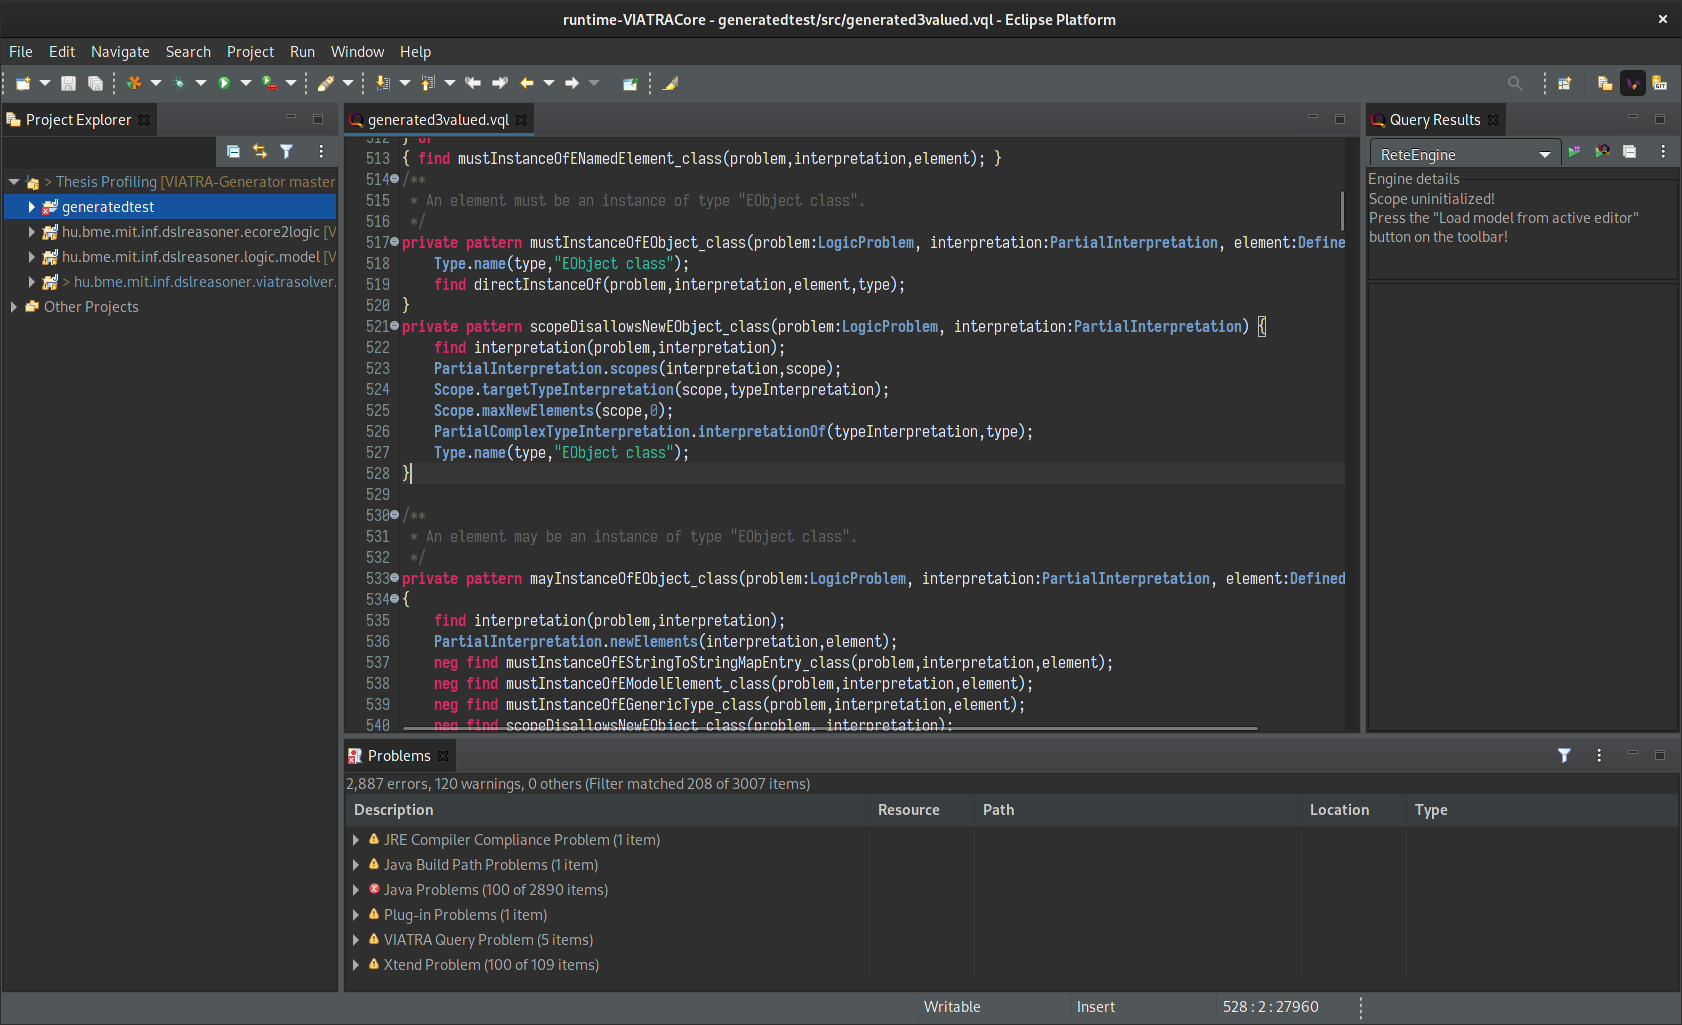
\includegraphics[width=150mm, keepaspectratio]{figures/eclipse-viatra.png}
\caption{The VIATRA Transformation Development perspective in Eclipse}
\label{fig:eclipse-viatra}
\end{figure}

\subsection{VIATRA Query Language (VQL)}
In VIATRA Query, we can write patterns that are matched on a loaded model. This
is done through a powerful domain-specific language (DSL) called the VIATRA
Query Language (VQL). The VIATRA Query plugins provide an editor with proper
syntax highlighting to make writing patterns easier.

Pattern syntax resembles Prolog in a way, that instead of writing functions, we
write statements, which are evaluated. The engine will try to calculate each
matching dataset for the pattern.

\begin{lstlisting}[frame=single]
pattern grandparentOf(grandchild : Person, grandparent : Person) {
    Person.parent(grandchild, parent);
    Person.parent(parent, grandparent);
}
\end{lstlisting}

In this pattern, we declare a grandparent of a person, as a parent of one of its
parents. This will match each grandparent-grandchild relation.

Patterns can have multiple declarations, and use other patterns.
If we separately track mothers and fathers instead of just parents, our patterns
may look like this.

\begin{lstlisting}[frame=single]
pattern parentOf(child : Person, parent : Person) {
    Person.mother(child, parent);
} or {
    Person.father(child, parent);
}

pattern grandparentOf(grandchild : Person, grandparent : Person) {
    find parentOf(grandchild, parent);
    find parentOf(parent, grandparent);
}
\end{lstlisting}

The last language feature I'll talk about is aggregation. You can use
aggregators for numeric results like \textbf{count}, \textbf{max}, \textbf{min},
and \textbf{sum}. In this snippet, the underscore means a parameter that is not
used in our pattern.

\begin{lstlisting}[frame=single]
pattern grandparentAmount(child : Person, amount) {
    amount == count find grandparentOf(child, _);
}
\end{lstlisting}

\subsection{Formulating constraints}
One can also provide model validation, by writing \textbf{constraint patterns}.
This raises an error if VIATRA finds any matches to that pattern. This can be
done by annotating our validation pattern.

\begin{lstlisting}[frame=single]
@Constraint(targetEditorId = "org.dfintha.familytree",
            severity = "error",
            message = "Person is both a parent and grandparent of someone.",
            key = {"parent"})
pattern bothParentAndGrandparent(person : Person, parent : Person) {
    find parentOf(person, parent);
    find grandparentOf(person, parent);
}
\end{lstlisting}

\section{Work environment}
\subsection{Eclipse Platform for VIATRA development}
VIATRA, as an Eclipse plugin is developed in Eclipse itself. As such, I needed
an Eclipse environment to develop it. Normally, this should be a straightforward
process, utilizing the Eclipse Oomph installer, but at the time I did my
research the installer didn't work as expected, so I had to install the required
plugins, and add the VIATRA source code to my environment manually.

The detailed steps on how to do this is is written down on the VIATRA project
website.

\subsection{YourKit Java Profiler}
Since the main issue we have to investigate is a slowdown, I had to use a
profiler software.

Profiler software examine various aspects of software execution, like how much
time did we spend in a function, or how many times a function was called, and
compile the measured data into snapshots, where the developer can analyze the
results.

During my thesis, I used the YourKit Java Profiler, for which the faculty
already owns a license.

After installing the profiler, I also had to install its Eclipse plugin, so I
could configure the profiler and start profiling of the software in Eclipse.

\chapter{Finding the cause of the editor slowdown}
\section{Problem description}
Users have complained, that the editor severely slows down during VQL pattern
editing, while working larger or more complex queries. To prove this statement,
I had to get a query that is both known to be slow and is correct. Fortunately,
there is an open-source VIATRA project, which contains a file, which causes
severe slowdowns, although, this generated file was not correct.

To create a test environment, I took that file, and fixed it in a new query
project, providing myself a clean slate for testing. The resulting file was over
5000 lines long and had a numerous amount of patterns referencing each other.
Editing this file caused 5-6 second hangups even with a moderately strong
computer.

\section{Profiling the query language editor}
\subsection{The profiling workflow}
First of all, I had to create a profiling workflow, which describes the steps
taken to profile the software. Following a fixed workflow ensures that snapshots
will not contain unrelated parts of the software execution, and that snapshots
will represent the same steps taken.

\begin{enumerate}
    \item{Start VIATRA in profiling mode, but without starting profiling itself.}
    \item{Wait for Eclipse to start and finish initial tasks.}
    \item{Open the query file, and wait for it to completely load, and highlight syntax.}
    \item{Navigate to a pattern, which we will manually duplicate.}
    \item{\textbf{Start profiling in the profiler software.}}
    \item{Manually type in the pattern again, with a different name.}
    \item{\textbf{Stop profiling in the profiler software, and save a snapshot.}}
    \item{Discard the changes we made in the file.}
    \item{Quit Eclipse.}
\end{enumerate}

\subsection{Profiling with default settings}
\subsection{Profiling without automatic update of target platform metamodels}
\subsection{Finding the critical part of metamodel updates}

\section{Type inference in VIATRA Query}
\subsection{Re-generating metamodels}
\subsection{Probable cause of the slowdowns}
\section{Conclusion}

\chapter{Optimizing query metamodel generation}
\section{TODO SOLUTION IDEA}
\section{Implementing the chosen solution}
\subsection{TODO SOLUTION STEPS}
\section{Comparing the optimized state with the original one}
\subsection{A first look}
\subsection{Original samples}
\subsection{Fixed samples}

\chapter{Applying changes to the main code repository}
\section{Writing documentation and tests}
\subsection{The asciidoc format}
\section{Opening a bug tracker ticket}
\section{Sending the changes to version control}
\section{Asking for code review}
\section{Integrating changes into the next VIATRA version}

% ---------------------------------------------------------------------------- %

\listoffigures\addcontentsline{toc}{chapter}{\listfigurename}
%\listoftables\addcontentsline{toc}{chapter}{\listtablename}

\addcontentsline{toc}{chapter}{\bibname}
\nocite{*} % FIXME remove
\bibliography{bib/mybib}

\label{page:last}
\end{document}
